\documentclass[a4paper,english,12pt]{article}
\usepackage{titlesec}

\usepackage[a4]{cc}
\usepackage{amsmath}
\usepackage[T1]{fontenc}
\usepackage[usenames,dvipsnames]{color}
\graphicspath{ {./images/} }
\usepackage[dvipsnames]{xcolor}
\titleformat*{\section}{\color{Brown}\normalfont\bfseries\Large}
\usepackage{prettyref}
\usepackage{amsthm}
\usepackage{amsmath}
\usepackage{amssymb}
\usepackage{float}
\usepackage{natbib}
\bibliographystyle{unsrtnat}
\PassOptionsToPackage{normalem}{ulem}
\usepackage{ulem}
\usepackage{mathptmx}
\usepackage{framed}
\usepackage{array}
\usepackage{csvsimple,longtable,booktabs}
\newlength{\mycolwidth}
\settowidth{\mycolwidth}{2cm} % widest entry


%\usepackage[unicode=true,pdfusetitle,
% bookmarks=true,bookmarksnumbered=false,bookmarksopen=false,
% breaklinks=false,pdfborder={0 0 1},backref=section,colorlinks=false]{hyperref}

\usepackage{pdfcomment}

%\newcommand{\dania}[1]{}
%\newcommand{\joyce}[1]{}
\newcommand{\chenc}[1]{\pdfcomment[author=Chen,color={1 0.5 0.5},subject={#1}]{#1}}
\newcommand{\dania}[1]{\pdfcomment[author=Dania,color={1 1 1},subject={#1}]{#1}}
\newcommand{\joyce}[1]{\pdfcomment[author=Joyce,color={1 0 1},subject={#1}]{#1}}
%\geometry{bindingoffset=2cm}


\usepackage{lipsum}

\hypersetup{colorlinks,
	linkcolor=red!95!black,%YellowOrange!85!black,
	citecolor=blue!85!black,
	pagecolor=blue!95!black,%
        urlcolor=magenta,filecolor=magenta,breaklinks,%
        dvips,bookmarks,bookmarksopen}

%\hypersetup{
%  linkcolor  = violet!\myshade!black,
%  citecolor  = YellowOrange!\myshade!black,
%  urlcolor   = Aquamarine!\myshade!black,
%  colorlinks = true
%}

\makeatletter
%\usepackage{pgfplots}
%\usepackage{tikz}
%\usepgfplotslibrary{external}
%\usetikzlibrary{external}
%\usepgflibrary{ plotmarks }
%\usetikzlibrary{arrows}
%\usetikzlibrary{plotmarks}
%\tikzexternalize[prefix = resource/]%, mode=list and make
%\tikzset{external/mode=graphics if exists}
%% the following forces redraw of all, if you reorder graphs
%tikzset{external/force remake}
\usepackage{microtype}
%
\usepackage{doi}
%\bibpunct{(}{)}{;}{a}{,}{,}

\renewcommand{\MakeUppercase}[1]{\color{green!50!black}\textsf{#1}}
%\usepackage{pdfsync}
\usepackage{amsfonts}
\usepackage{amscd}
\usepackage{bm}
\usepackage{euler}
\usepackage{url}
%\graphicspath{resource/}
%\graphicspath{./resource/}
\newcommand{\pde}{{\textsc{pde}}}
\newcommand{\res}{{\operatorname{Res}}}
\newcommand{\D}[2]{\frac{\partial #1}{\partial #2}}
\newcommand{\DD}[2]{\frac{\partial^2 #1}{\partial #2^2}}
\newcommand{\pp}{{}+}
\newcommand{\Ord}{\mathcal{O}}
\newcommand{\LL}{\mathcal{L}}
\newcommand{\ode}{{\textsc{ode}}}
\newcommand{\cL}{\mathcal{L}}
\newcommand{\lhs}{{\textsc{lhs}}}
\newcommand{\rhs}{{\textsc{rhs}}}
\newcommand{\dd}[2]{\frac{\partial #1}{\partial #2}}

\usepackage{listings}
\lstset{escapeinside={(*@}{@*)}}
\usepackage{inconsolata}
\usepackage{textcomp}
%% Actual colors from idlelib/config-highlight.def --> corrected to ``web-safe''
%% strings  = #00aa00 / 0,170,0      (a darker green)
%% builtins = #900090 / 144,0,144    (purple-ish)
%% keywords = #FF7700 / 255,119,0    (quite close to plain `orange')
%% Corrected to ``web-safe''
\definecolor{purple2}{RGB}{153,0,153} % there's actually no standard purple
\definecolor{green2}{RGB}{0,153,0} % a darker green

\lstdefinestyle{python-idle-code}{%
  language=Python,                   % the language
  showspaces=false,
  showtabs=false,
  breaklines=true,
  showstringspaces=false,
  breakatwhitespace=true,
  basicstyle=\normalsize\ttfamily,   % size of the fonts for the code
  % Color settings to match IDLE style
  keywordstyle=\color{orange},       % core keywords
  keywordstyle={[2]\color{purple2}}, % built-ins
  stringstyle=\color{green2},
  commentstyle=\color{red},
  upquote=true,                      % requires textcomp
}
%\lstloadlanguages{Python}
\lstset{
  style={python-idle-code},
  showstringspaces=false,  % true by default for python
  % tabsize=4,
}
\lstset{
float=table,
stringstyle=\color{orange},
basicstyle=\color{black}\footnotesize\ttfamily,
numbers=left,
numberstyle=\tiny\color{brown},
%numberstyle=\small,
numbersep=8pt,
%frame = leftline,
breaklines=true,
firstnumber=1,
language=python,
numberstyle=\tiny\color{brown},
keywordstyle=\color{blue},
commentstyle=\color{green!50!black}}

% These are recommended by Rob J Hyndman (2011)
% \footnote{\url{http://robjhyndman.com/researchtips/latex-floats/}}
\setcounter{topnumber}{2}
\setcounter{bottomnumber}{2}
\setcounter{totalnumber}{4}
\renewcommand{\topfraction}{0.85}
\renewcommand{\bottomfraction}{0.85}
\renewcommand{\textfraction}{0.15}
\renewcommand{\floatpagefraction}{0.7}
\renewcommand{\lstlistingname}{Algorithm}
\usepackage[UKenglish]{babel}
%\includeonly{chapter3/chapter3}
\title{Assignment 1---Group: }
\author{Chen Chen (480458339), Xiaodan Gan(440581983) \\
	Xinyue Wang (440359463)}
\makeatother

\begin{document}
%\listofpdfcomments
\maketitle
\begin{abstract}
\emph{This project numerically compares the robustness of two nonnegative matrix factorisation (\textsc{nmf}) algorithm \citep{lee2001algorithms} based on multiplicative update rules when contaminated by large magnitude Gaussian, Poisson and Salt \& Pepper noise. Section~\ref{chp3} briefly reviews relevant work in the field of \textsc{nmf}, which found these multiplicative update rules are very sensitive to initialisation. Section~\ref{chapter2} describes the two algorithms and their theoretical properties, proposes a solution to make the multiplicative update rules less sensitive to initialisation, and details the statistical tools we used to compare the robustness of the two algorithm. Our simulation results in Section~\ref{chapter4} agree with the theoretical properties of the two algorithms. Future work involves embedding the proposed multiple initialisations into the \textsc{nvidia} \textsc{gpu} based parallel-programming model.}
\end{abstract} 

\tableofcontents{}

\section{Introduction\label{chapter1}}
%Briefly introduce \textsc{nmf}, applications
Non-negative matrix factorization (\textsc{nmf}) is a matrix decomposition technique that approximates a multivariate data matrix by two lower dimensional non-negative matrices as follows:
\begin{equation}
  vv
\end{equation}
As \textsc{nmf} only allows additive, non-subtractive combination of matrix factors, it is applicable to an extensive range of domain \chenc{sorry but I do not understand}. \citet{lee1999learning} suggest that \textsc{nmf} is useful for image processing problems including facial recognition. Specifically, \textsc{nmf} generates two matrices $W$ and $H$ which are often referred as the basis images and weights. This is because the observed image $V$ is approximated by a linear combination of $W$ and $H$. This property also distinguishes \textsc{nmf} from other traditional image processing methods such as principal components analysis (\textsc{pca}) and $K$-means clustering \chenc{$K$ means is not only a image processing technique, delete}. \citet{guillamet2002non} demonstrate that \textsc{nmf} is more robust to corrupted images than \textsc{pca}.
Moreover, \textsc{nmf} is also applicable to text mining such as semantic analysis. More generally, \textsc{nmf} is useful to discover semantic features of an article by counting the frequency of each word than approximating the document from a subset of a large array of features \citep{lee1999learning}.

Researchers proposed many \textsc{nmf} algorithms. \citet{lee2001algorithms} first proposes ``multiplicative update rules'' to minimise Euclidean distance or Kullback-Leibler divergence between the original matrix and its approximation. Although this algorithm is easy to implement and have reasonable convergent rate \citep{lee2001algorithms}, it may fail on seriously corrupted dataset which violates its assumption of Gaussian noise or Poisson noise, respectively \citep{guan2017truncated}.  To improve the robustness of \textsc{nmf}, many methods have been proposed. Lam ????? \chenc{no bib file}(2008) proposes ${L_1}$-norm based \textsc{nmf} to model noisy data by a Laplace distribution which is less sensitive to outliers. However, as $L_1$-norm is not differentiable at zero, the optimization procedure is computationally expensive. \citet{kong2011robust} proposed an \textsc{nmf} algorithm using $L_{21}$-norm loss function which is robust to outliers. The updating rules used in $L_{21}$-norm \textsc{nmf}, however, converge slowly because of a continual use of the power method \citep{guan2017truncated}.

In practice, face images could be easily corrupted during data collection by large magnitude noise. Corruption may result from lighting environment, facial expression or facial details. An \textsc{nmf} algorithm that is robust to large noise is desired for real-world application. Therefore, the objective of this project is to analyse the robustness of \textsc{nmf} algorithms on corrupted dataset. We implement two \textsc{nmf} algorithms on real face image datasets, \textsc{orl} dataset and Extended YaleB dataset. The face images are contaminated by artificial noises.

Plan:
...




\section{Related work}
Researchers proposed many \textsc{nmf} algorithms. As the objective function of \textsc{NMF} is non-convex, for which the traditional gradient decent method is not applicable, \citet{lee2001algorithms} first proposes to algorithms which minimises Euclidean distance or Kullback-Leibler divergence (\textsc{KLD}) between the original matrix and its approximation. Although this algorithm is easy to implement and have reasonable convergent rate \citep{lee2001algorithms}, it may fail on seriously corrupted dataset which violates its assumption of Gaussian noise or Poisson noise, respectively \citep{guan2017truncated}. Moreover, \citet{yang2011kullback} indicate that \textsc{KLD} is sensitive to the inital value of matrix factors and requries many iterations to retrieve from wrong initial values.  To improve the robustness of \textsc{nmf}, many methods have been proposed. \citet{lam2008non} proposes ${L_1}$-norm based \textsc{nmf} to model noisy data by a Laplace distribution which is less sensitive to outliers. However, as $L_1$-norm is not differentiable at zero, the optimization procedure is computationally expensive. \citet{kong2011robust} proposed an \textsc{nmf} algorithm using $L_{21}$-norm loss function which is robust to outliers. The updating rules used in $L_{21}$-norm \textsc{nmf}, however, converge slowly because of a continual use of the power method \citep{guan2017truncated}.

Apart from different loss functions, several optimization methods were proposed to improve the performance of \textsc{nmf}. After \citet{lee2001algorithms} proposed  multiplicative update rules \textsc{mur}, \citet{ lin2007convergence} proposed a modified \textsc{mur} which guaranteed the convergence to a stationary point. This modified \textsc{mur}, however, did not improve the convergence rate of traditional \textsc{mur} \citep{guan2012nenmf}. Moreover, as \textsc{mur} is not able to shrink all entries in matrix factors to zero, \citet{berry2007algorithms} proposed a projected nonnegative least square (\textsc{pnls}) method to overcome this problem. Although, in each nonnegative least square (\textsc{nls}) subproblem, the least squares solution is directly projected to the negative quadratic, \textsc{pnls} does not guarantee convergence \citep{guan2012nenmf}. In contrast to these gradient-based optimization methods, \citet{kim2008nonnegative} presented an active set method \textsc{as} which divides variables into two sets, free set and active set and update free set in each iteration by solving unconstrained equation. Even though \textsc{as} has good convergence rate, it assumes strictly convex in each \textsc{nls} subproblem \citep{kim2008nonnegative}.

%!TEX root = report.tex
\section{Methods \label{chapter2}}
%\subsection{Noise Design}
Some carefully designed \textsc{nmf} are robust to various noises. These robust algorithms aim to significantly reduce the amount of noise while preserving the edges without blurring the immage \citep{barbu2013variational}. %Figure~\ref{noises} shows three kinds of noises we designed, including Gaussian noise, Poisson noise, and Salt \& Pepper noise.

\subsection{NMF and Gaussian noise}
\textbf{Gaussian noise} is a noise with a probability density function being normal with mean zero. \citet{lee2001algorithms} propose the first \textsc{nmf} with the objective function between imaga~$V$ and its \textsc{nmf} factorisation~$W$ and~$H$ being
\begin{equation}
  \left\Vert V-WH \right\Vert= \sum_{ij} \left[V_{ij}-(WH)_{ij}\right]^2.\label{eq:obnmf}
\end{equation}
To minimise this object function of least square, \citet{lee2001algorithms} prove the convergence of the multiplication update rule
\begin{equation}
H_{jk}\leftarrow H_{jk}\frac{(W^{T}V)_{jk}}{(W^{T}WH)_{jk}} \text{ and } W_{ij}\leftarrow W_{ij}\frac{(VH)_{ij}}{(WHH^{T})_{ij}}.\label{eq:nmf}
\end{equation}
Here, $()_{ij}/()_{ij}$ denotes elementwise division of the two matrix. \citet{liu2015performance} shows this \textsc{nmf} algorithm minimises Gaussian.

\subsection{KLNMF and Poisson noise}
\textbf{Poisson noise} or shot noise is a type of electronic noise that
occurs when the finite number of particles that carry energy,
such as electrons in an electronic circuit or photons in an optical
device, is small enough to give rise to detectable statistical
fluctuations in a measurement.
\citet{lee2001algorithms} suggest that \textsc{klnmf} is a algorithm that minimising the Kullback-Leibler divergence
\begin{eqnarray}
  D(V||WH)&=&\sum_{ij}\left(V_{ij}\log\frac{V_{ij}}{\left(WH\right)_{ij}}-V_{ij}+\left(WH\right)_{ij}\right)\nonumber\\
          &=&\sum_{ij}\left(-V_{ij}\log\left(WH\right)_{ij}+\left(WH\right)_{ij}+C(V_{ij})\right).\label{eq:klobj}
\end{eqnarray}
where $C(V_{ij})=V_{ij}\log V_{ij}-V_{ij}$. $C(V_{ij})$ is a function of the observed image matrix~$V$ only.
\citet{lee2001algorithms} also suggest a multiplication update rule to find as the optimisation procedure of \textsc{klnmf}
\begin{equation}
H_{jk}\leftarrow H_{jk}\frac{\sum_{i}W_{ij}V_{ik}/(WH)_{jk}}{\sum_{i'}W_{i'j}} \text{ and } W_{ij}\leftarrow W_{ij}\frac{\sum_{k}H_{jk}V_{ik}/(WH)_{jk}}{\sum_{k'}H_{ik'}}. \label{eq:klnmf}
\end{equation}
As this original image matrix~$V$ is observed, minimising this Kullback-Leibler divergence~\eqref{eq:klobj} is equivalent to minimising
\begin{equation*}
  \sum_{ij}\left(-V_{ij}\log\left(WH\right)_{ij}+\left(WH\right)_{ij}+C(V_{ij})\right).
\end{equation*},
for arbitrary bounded function~$C(V_{ij})$. Taking exponential of the negative of this score function, the problem transforms to maximising the following likelihood function
\begin{equation*}
L(WH|V)=\prod_{ij}\left(\left(WH\right)_{ij}^{V_{ij}}e^{-\left(WH\right)_{ij}}+C(V_{ij})\right).
\end{equation*}
Choosing constant $C(V_{ij})$ to be $-\log V_{ij}!$ gives
\begin{equation*}
L(WH|V)=\prod_{ij}\left(\frac{\left(WH\right)_{ij}^{V_{ij}}e^{-\left(WH\right)_{ij}}}{V_{ij}!}\right).
\end{equation*}
Hence, the probability density function of each element of the original matrix~V is Poisson
\begin{equation*}
P(V_{ij})=\frac{\left(WH\right)_{ij}^{V_{ij}}e^{-\left(WH\right)_{ij}}}{V_{ij}!}
\end{equation*}
is a sufficient condition to yield this likelihood. Hence \textsc{klnmf} is most suitable for images with Poisson noise.

\subsection{Preprocess}
We did not preprocess the images because both of \textsc{nmf} and \textsc{klnmf} are scale sensitive, because both objective functions~\eqref{eq:obnmf} and~\eqref{eq:klobj} varies when original matrix~$V$ and result matrices~$W$ and~$H$ scale proportionally, i.e. for $\lambda$ real, $D(V||WH)\neq D(\lambda V||\lambda WH)$. To overcome this issue, we could have normalise the matrices~$W$ and~$H$ in each iteration \citep{scaless}, but it will result in a even slower computation.

\subsection{Gaussian and Poisson are asymptotic equivalent}
 We design an Gaussian noise and a Poisson noise with different magnitude.
 Poisson distribution with parameter~$\lambda$ (integer) is equivalent to the sum of $\lambda$ Poisson distributions with parameter~$1$ \citep[][p. 45]{Walck:1996cca}.
 Hence for $\lambda$ large, Central Limit Theorem implies that Poisson distribution with parameter~$\lambda$ is well approximated by $N(\lambda,\lambda)$.
 When applying Poisson noise to an image, we do not have degree of freedom to choose any parameter.
 The variance is the magnitude of the pixels. To compare the robustness of \textsc{klnmf} with \textsc{nmf} with different noise, we choose the variance of Gaussian noise to be the different from the magnitude of the pixel, that is, $N(0,\operatorname{Var})\neq N(0,V)\approx \operatorname{Poi}(V)-V$.
 Figure~\ref{noise} visualises the similarity of Poisson distribution and Normal distribution with parameter~$V=40$. To overcome this issue, the Gaussian noise we use should be larger or smaller variance in comparison with the mean of the images. We choose the variance of the noise to be $80$.
\begin{figure}
  \centering
  % Requires \usepackage{graphicx}
  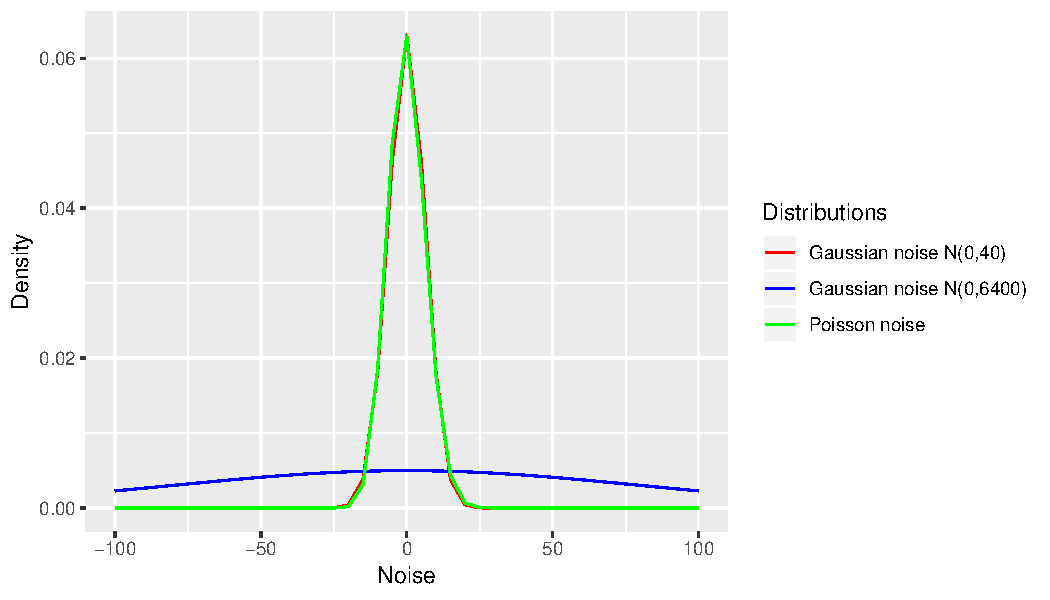
\includegraphics[scale=1]{resource/noise}\\
  \caption{Compare a Gaussian noise~$N(0,40)$ with Poisson noise $\operatorname{Poi}(40)-40$. They two distributions are asymptotically equivalent and have similar density functions.}\label{noise}
\end{figure}

\subsection{Salt \& Pepper noise}
Apart from Gaussian and Poisson noises, we also test our two algorithms on the commonly seen \textbf{Salt \& Pepper noise} noise. The noise presents itself by having dark pixels in bright regions and bright pixels in dark regions \citep{sampat2005computer}.

\subsection{Multiple initial estimates assure the algorithms stable}
As discussed in the section of related work,
The problem of nonnegative matrix factorization is not a convex problem.
Hence the results update rules~\eqref{eq:nmf} and~\eqref{eq:klnmf} coverage to may be local minima instead of global minima, depending on the initial approximation.
Our task was to compare the robustness of the algorithm and we do not want the instability of our algorithms to affect our comparison.
To address this issue, we implement several (i.e. $n$) initial estimates for each matrix factorization problem.
We use the factorized matrices~$W$ and~$H$ corresponding to the least residual~\eqref{eq:obnmf} and~\eqref{eq:klobj}, for \textsc{nmf} and~\textsc{klnmf}, algorithms respectively, as the final result of factorization.
This design of multiple starting point improves the stability of of algorithm, but it requires more computational power. To improve the computational speed, we make the number~$n$ equal to the number of cores of the \textsc{cpu}. We assign each of the $n$ initial estimates randomly with an uniform distribution. Then these each of the $n$ initial estimates are assigned to a different core of the \textsc{cpu}. This boost the \textsc{cpu} utilisation to 100\% instantly and improved the computational speed by 70\% on the \textsc{orl} data. The following part of our code implements this idea of parallel computing.
\begin{lstlisting}[caption=Centring image data, label=matn1]
args = zip(repeat(V,ncpu), repeat(r,ncpu), repeat(niter[name2],ncpu), repeat(min_error[name2],ncpu))
result = pool.starmap(algo, args)
\end{lstlisting}
where \texttt{algo} is the \textsc{nmf} algorithm and \texttt{niter} is the number of iterations. We use Chen's 16-thread Xeon high performance computer to run this algorithm.


\subsection{KLNMF requires more iterations}
\textsc{klnmf} converges slower than \textsc{nmf}. We made the plot of the logarithm of residual~\eqref{eq:obnmf} and~\eqref{eq:klobj} with respect to the logarithm of the number of iterations. We measured the slope of the log-log plot for both algorithms and found that the slope of the \textsc{nmf} residual plot is $2.5$ times as that of the \textsc{klnmf} plot (Figure~\ref{error}). This estimates that the rate of convergence of \textsc{nmf} is $2.5$ faster than \textsc{klnmf}. As a result, we set the number of iterations as $500$ and $1200$ for \textsc{nmf} and \textsc{klnmf} algorithms, respectively (i.e. roughtly $2.5$ more iterations).
 \begin{figure}
  \centering
  % Requires \usepackage{graphicx}
  \includegraphics[scale=.8]{error}\\
  \caption{Residual of objective function~\eqref{eq:obnmf} and~\eqref{eq:klobj} versus the number of iterations. \textsc{nmf} converges more than twice faster than \textsc{klnmf}.}\label{error}
\end{figure}

\subsection{Evaluation metrics and their confidence intervals \label{ci}}
The assignment instruction asks us to compare the performance of \textsc{nmf} and \textsc{klnmf} by using evaluations metrics including Relative Reconstruction Errors (\textsc{rre}), Average Accuracy (\textsc{aa}), Normalized Mutual Information (\textsc{nmi}). The instruction states the formulae of these metrics. However, to systematically compare the metrics, we construct an 95\% confidence interval for any metric (e.g. \textsc{rre}) by bootstrapping percentile confidence interval. The idea of bootstrapped  is straightforward---we resample a subset of $40$ samples among the sample space of $80$ simulations and calculate the mean. We repeat this process $1000$ times. The $2.5\%$ and $97.5\%$ percentiles of the $80$ resampled means are then the bootstrapping percentile confidence interval
\begin{equation}
(\textsc{rre}^*_{2.5}, \textsc{rre}^*_{97.5}), \label{eq:boot}
\end{equation}
where $\textsc{rre}^*_{\alpha}$ is the $\alpha$ percentile of the bootstrapped distribution from our sample space with $80$ simulations.  We run $80$ simulations so that the confidence interval we construct is precise.

Boostrapping does not require the sample space follows specific distributions. We apply this nonparametric method to construct confidence interval here because we do not have the knowledge about the specific distributions of these three metrics.

\subsection{Statistical method compares the robustness of algorithms}
We implement Kolmogorov-Smirnov test to test the hypothesis that the algorithms~\textsc{nmf} and~\textsc{klnmf} have different robustness. Again Kolmogorov-Smirnov test is distribution free, so we do not need to know the distributions of the evaluation metrics.

Let $\textsc{rre}_i$ denote the \textsc{rre} generated from our \textsc{nmf} algorithm by the $i$th simulation. Define the empirical distribution of a sample set generated by algorithm~$\alpha$, perhaps the $80$ \textsc{rre} results, as
\begin{equation}\label{epdf}
  \hat{F}_{\alpha}(x)=\frac{1}{n}\sum_{i=1}^{80}1_{\textsc{rre}_i \leq x}.
\end{equation}
The test statistic is the supremum among the differences of the empirical distribution generated using definition~\eqref{epdf} \citep{Walck:1996cca}
\begin{equation}\label{teststatistic}
D=\sup _{x}\left|F_{\alpha_2}(x)-F_{\alpha_2}(x)\right|.
\end{equation}
We compare the test statistics~$D$ with the critical value of $0.215$, which corresponds to $80$ samples and a 95\% of confidence level. We reject the null hypotheses that the two algorithms produce similar \textsc{rre} (or other evaluation metrics) with 95\% confidence level if the test statistics~$D>0.215$. The technique is extended to compare \textsc{aa} and \textsc{nmi}.
%\csvautobooktabular{{"../results/statistics".csv}}
%\subsection{Preprocessing}
%We apply global centring and local centring to preprocess the image data~\texttt{Vhat}
%\begin{lstlisting}[caption=Centring image data, label=matn1]
%n_samples = len(Vhat)
%# global centering
%Vhat = Vhat - Vhat.mean(axis=0)
%# local centering
%Vhat -= Vhat.mean(axis=1).reshape(n_samples, -1)
%Vhat -= Vhat.min()
%\end{lstlisting}


\section{Experiments}\label{chapter4}

\subsection{Dataset}
We illustrate our two \textsc{nmf} algorithms on two real-world face image datasets: \texttt{ORL} and \texttt{CroppedYaleB} (\citet{belhumeur1997eigenfaces}).
Both \texttt{ORL} and \texttt{CroppedYale} datasets contain multiple images of distinct subjects with various facial expression, lighting condition, and facial details.
Images in ORL are cropped and resized to $92 \times 112$ pixels. We further rescale it to $30 \times 37$ pixels. Similarly, we reduce the size of images in \texttt{CroppedYale} to $42 \times 48$ pixels.
For each dataset, we flatten the image matrix into a vector and append them together to get a matrix $V$ with shape $d\times n$ where integer~$d$ is the number of pixels in one image and integer~$n$ is the number of images. In each epoch, we use 90\% of data.

\subsection{Noise}
We implement three kinds of noises including Gaussian noise, Poisson noise and Salt \& Pepper noise.
\subsubsection{Gaussian Noise}\label{sec:gau}
We design the Gaussian noise by a normal distribution with a mean of $0$ and a standard deviation of $80$ (Algorithm~\ref{gau}). The \texttt{ORL} dataset has a global pixel mean of $40$ and the \texttt{CroppedYale} dataset has that of $70$. Hence the designed Gaussian noise contaminates the images significantly. We choose the standard deviation to be $80$ so that our Gaussian noise is less likely to coincident with the designed Poisson noise. To satisfy the nonnegative constant, negative value in the contaminated image is set to zero.
\begin{lstlisting}[caption= Gaussian Noise Design, label=gau]
def normal(subVhat):
    """Design a Gaussian noise."""
    V_noise = np.random.normal(0, 80, subVhat.shape) #* np.sqrt(subVhat)
    V = subVhat + V_noise
    V[V < 0] = 0
    return V, V_noise
\end{lstlisting}


\subsubsection{Poisson Noise}\label{sec:poi}
The Poisson noise is not additive and has no hyperparameters to be set. Unlike Gaussian noise, contaminated images are drawn directly from Poisson distributions with parameters set to be pixel values. Then, the Poisson noise is calculated from the difference between the contaminated image and the original image, as discussed in Section~\ref{chapter2} and demonstrated in algorithm~\ref{poi}.
\begin{lstlisting}[caption= Poisson Noise Design, label=poi]
def possion(subVhat):
    """Design a Possion noise."""
    V = np.random.poisson(subVhat)
    V_noise = V-subVhat
    return V, V_noise
\end{lstlisting}


\subsubsection{Salt \& Pepper Noise}\label{sec:sal}
% JOYCE please add here
Salt \& Pepper noise is added by drawing random integers from the discrete uniform distribution of the interval $[0, 255)$ . We find the bright places in generated image and replace pixel values in the same place of the original image with the brightest value. Similarly, we also find the dark pixels in the  images and replace pixel values in the same place of original image with the  darkest pixel value. In this case, we set the pixels whose values are greater than or equal to 230 as bright pixels and pixels whose value being less than or equal to 20 as dark pixels.
\begin{lstlisting}[caption= Salt and Pepper Noise Design, label=salt]
def salt_and_pepper(subVhat):
"""Design a salt and pepper noise where make some pixel value zeros."""
  V_noise = np.random.randint(low=0, high=255, size=subVhat.shape, dtype=int)
  V = subVhat.copy()
  V[V_noise <= 20] = 0
  V[V_noise >= 230] = 255
  return V, V_noise
\end{lstlisting}

\subsection{Experiment Setup}

We apply two algorithms (\textsc{nmf} and \textsc{klnmf}) with four categories of noises (no noise, Gaussian noise, Poisson noise and Salt \& Pepper noise), which results in eight combinations in each epoch. In each epoch, we randomly select 90\% of samples to train NMF algorithms and evaluate three metrics on reconstructed images. The training will terminate when the error reaches the minimum error, or the maximum iteration is reached. The minimum error and maximum iteration are hyperparameters which we learn from iterative experiments. Our code saves the learning errors versus the number of iterations so that we could draw the plot and observe the convergence of the learning process. We increase the number of epochs and calculate the average metrics and confidence intervals.


\subsection{Experiments Results}
Figure~\ref{noisesnmff} and~\ref{noisesklnmff} visualise the original image, designed noises, corrupted images and reconstructed images from left to right. From top to bottom, the four rows correspond to no noise, Gaussian noise discussed in Section~\ref{sec:gau}, Poisson noise discussed in Section~\ref{sec:poi} and Salt \& Paper noise discussed in Section~\ref{sec:sal}.
The first row of Figure~\ref{noisesnmff} and~\ref{noisesklnmff} show both algorithms reconstructed the original image well without artificial noise and with Poisson noise.
\begin{figure}
	\centering
	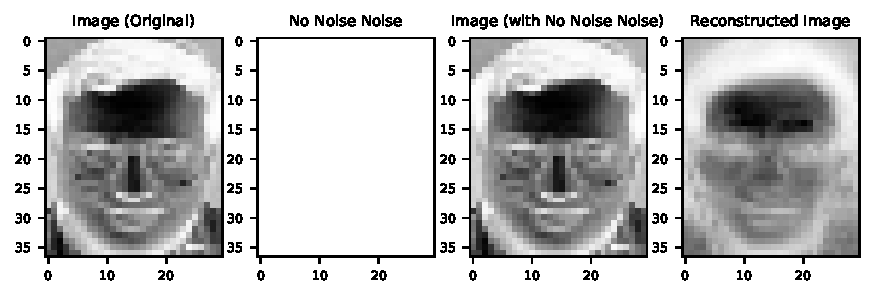
\includegraphics[scale=.9]{Result_Multiplication_Euclidean_No_Noise_Comparison}\\
	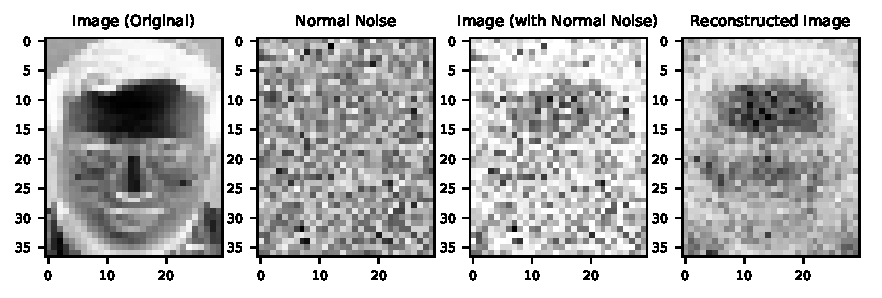
\includegraphics[scale=.9]{Result_Multiplication_Euclidean_Normal_Comparison}\\
	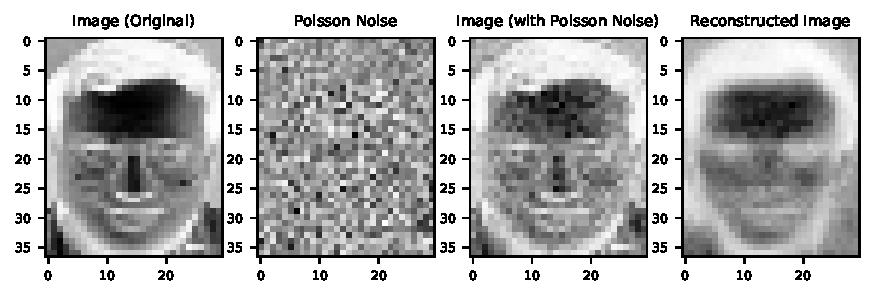
\includegraphics[scale=.9]{Result_Multiplication_Euclidean_Poisson_Comparison}\\
	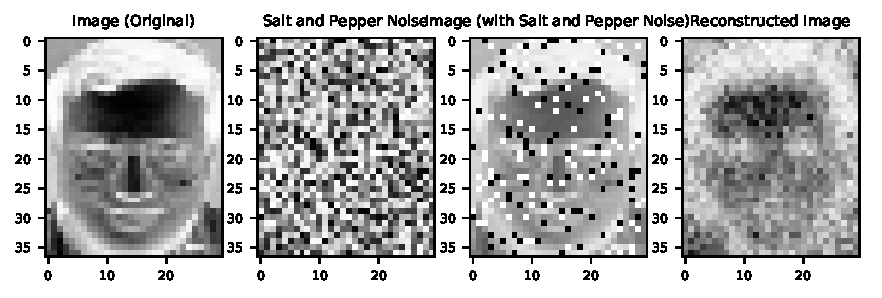
\includegraphics[scale=.9]{Result_Multiplication_Euclidean_Salt_and_Pepper_Comparison}
	\caption{The reconstructed image by \textbf{nmf}. The original images (Column~1) are combined with noises (Column~1) including Gaussian Noise with Variance~$80$ (Row~2), Poisson Noise (Row~3), and Salt \& Pepper Noise (Row~4). The corrupted images are shown in Column~3. The reconstructed images are shown in (Column~4). The reconstruction with no noise is shown in Row~1.}\label{noisesnmff}
\end{figure}
\begin{figure}
	\centering
	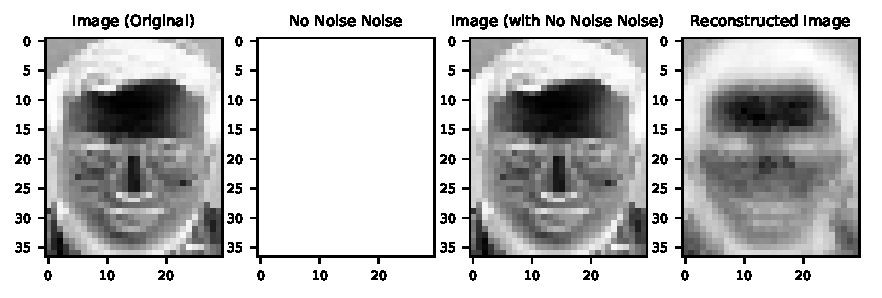
\includegraphics[scale=.9]{Result_Multiplication_KL_Divergence_No_Noise_Comparison}\\
	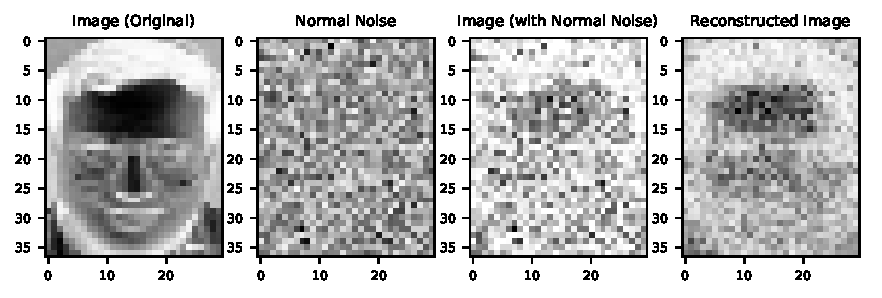
\includegraphics[scale=.9]{Result_Multiplication_KL_Divergence_Normal_Comparison}\\
	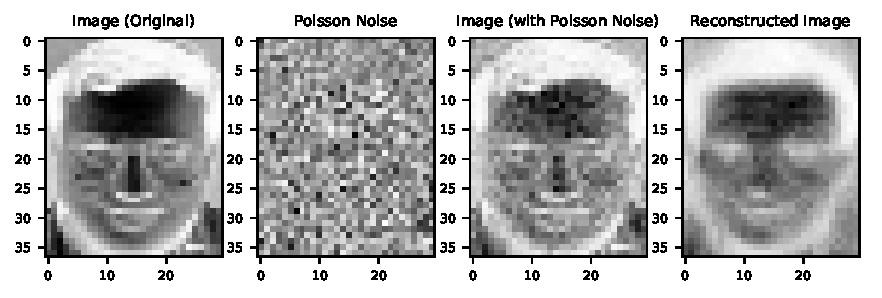
\includegraphics[scale=.9]{Result_Multiplication_KL_Divergence_Poisson_Comparison}\\
	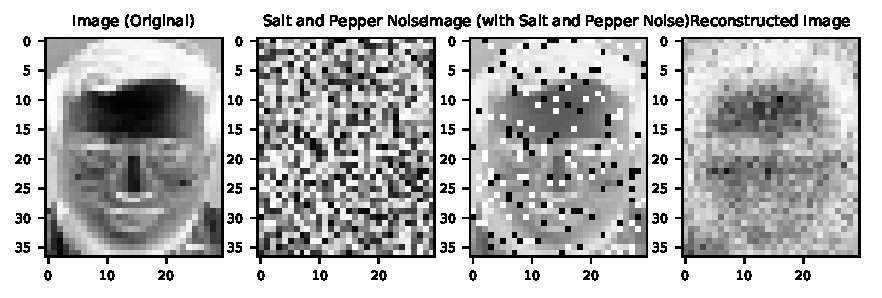
\includegraphics[scale=.9]{Result_Multiplication_KL_Divergence_Salt_and_Pepper_Comparison}
\caption{The reconstructed image by \textbf{klnmf}. The original images (Column~1) are combined with noises (Column~1) including Gaussian Noise with Variance~$80$ (Row~2), Poisson Noise (Row~3), and Salt \& Pepper Noise (Row~4). The corrupted images are shown in Column~3. The reconstructed images are shown in (Column~4). The reconstruction with no noise is shown in Row~1.}\label{noisesklnmff}
\end{figure}
However, when the noise is large (the second and last rows in Figure~\ref{noisesnmff} and~\ref{noisesklnmff}), the quality of reconstructed images looks marginally better than the contaminated images.
This result is consistent with \citet{guan2017truncated}, who assert that \textsc{nmf} may fail to handle extremely corrupted images when we violate the assumptions on the distributions of noise.
Moreover, the difference between images generated by \textsc{nmf} and \textsc{klnmf} are not visually significant.
Hence, we implement the statistical hypothesis test to compare of \textsc{rre}s of the two algorithms.

Substitute \href{https://raw.githubusercontent.com/JoyceXinyueWang/nmf_raw_data/master/raw_result_acc.csv}{\textsc{rre} results} (Figure~\ref{histo}) from $80$ Monte-Carlo simulations of the two algorithms into Kolmogorov-Smirnovs test~\eqref{teststatistic} gives test statistics~$D=1, 1 ,0.6625$ with no noise, Gaussian noise, and Poisson noise, for the \texttt{ORL} dataset. These three test statistics are all much greater than the critical value~$0.215$. Hence there are strong statistical evidences that the performance of \textsc{nmf} and \textsc{klnmf} are different in these three problems. For salt and Pepper noise, test statistic~$D=0.2125<0.215$, hence we fail to conclude that the two methods have different robustness against Salt and Pepper noise. Further, one tail Kolmogorov-Smirnov test concludes that \textsc{klnmf} performs better reconstructing the original image with no noise and is more robust Poisson noise. 
In contrast, \textsc{nmf} is more robust against Gaussian noise, even with only $500$ iterations ($1200$ for \textsc{klnmf}).
\begin{figure}
{\centering
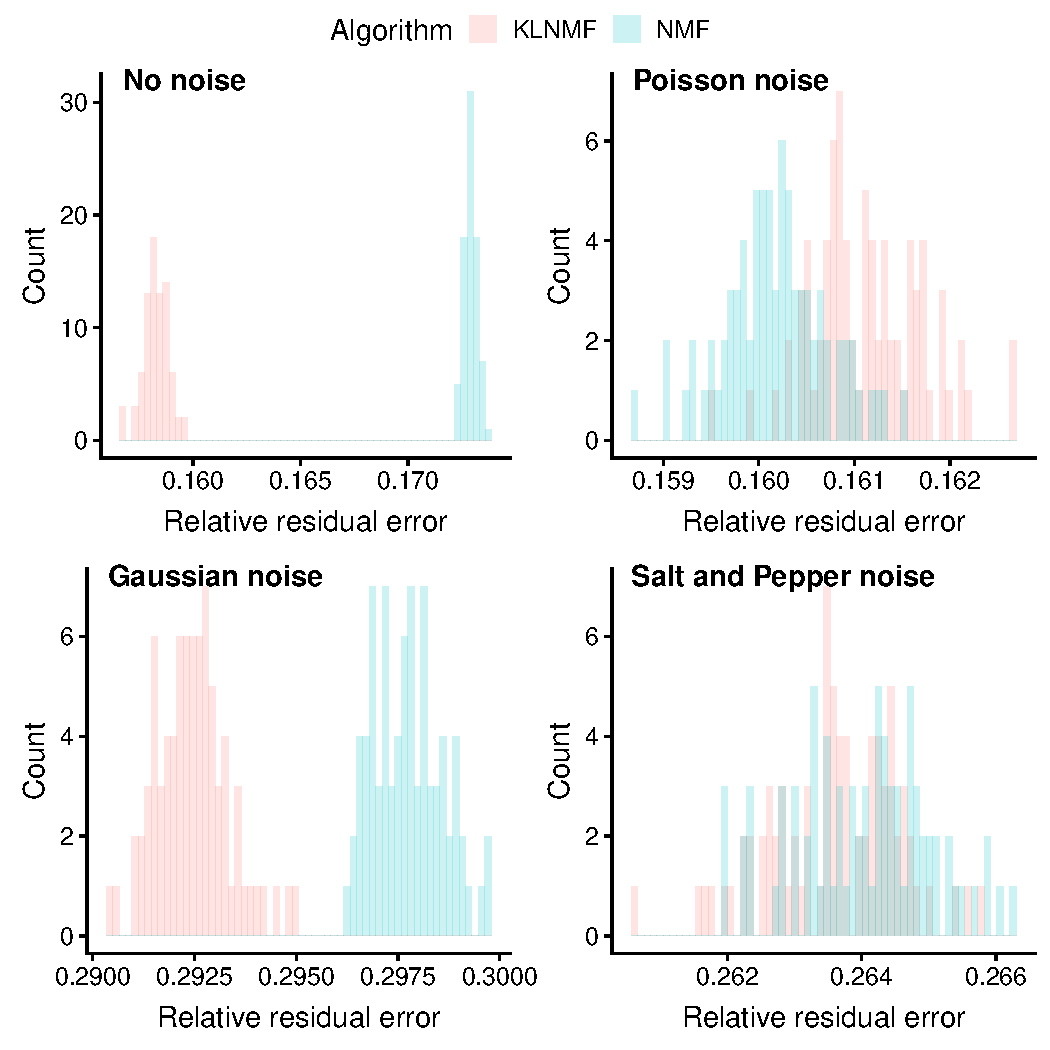
\includegraphics[scale=0.8]{histo}
\caption{Histogram of \textsc{rre} results from 80 Monte-Carlo simulations. Blue bars correspond to \textsc{nmf, and the pink bars correspond to \textsc{klnmf}. The types of noise are labelled in the plot. The visualisation agrees with our statistical analysis.}
\label{histo}}}
\end{figure}
Theoretical results discussed in Section~\ref{chapter2} suggest \textsc{nmf} is more robust against Gaussian noise whereas \textsc{klnmf} is more robust against Poisson noise. Our experimental results concluded from Kolmogorov-Smirnovs hypothesis tests agree with these theoretical results. Further, as both of the algorithms are not designed for Salt and Pepper noise, they have a similar performance against it.

These results can be observed by directly reading whether the confidence intervals overlap in table~\ref{tab:ci}. Also, the statistical results agree with the visualisation in Figure~\ref{histo},~\ref{noisesnmff} and~\ref{noisesklnmff}. These results also agree with our intuition---although the differences in the robustness of the two algorithms are small, the even smaller variances in the \textsc{rre} results make them statistically different under Poisson and Gaussian noise (Figure~\ref{histo}).

In terms of the \texttt{CroppedYale} dataset, results from hypothesis tests show that \textsc{nmf} performs uniformly better than \textsc{klnmf}, suggesting more iterations are required on \textsc{klnmf} to compare these two algorithms fairly. We fail to do so because the dataset is much larger than \texttt{ORL} and our multiplicative update rules, especially for \textsc{klnmf} converge too slow.

\begin{table}
\caption{Average of evaluations metrics over 80 Monte-Carlo simulations using the \texttt{ORL} dataset. The 95\% confidence intervals are calculated using bootstrap.}
\hspace{-1cm}{\small
\label{tab:ci}\begin{tabular}{l|lll}
 \hline
\texttt{ORL} dataset & \textsc{rre} & \textsc{acc} & \textsc{nmi}\tabularnewline
 \hline
\textsc{nmf} no noise & 0.1583 (0.1581, 0.1584) & 0.7364 (0.731, 0.742) & 0.8536 (0.8506, 0.8567)\tabularnewline

\textsc{nmf} Gaussian noise & 0.2925 (0.2922, 0.2927) & 0.447 (0.4423, 0.4521) & 0.6212 (0.6176, 0.6247)\tabularnewline

\textsc{nmf} Poisson noise & 0.1611 (0.161, 0.1613) & 0.7313 (0.7262, 0.7367) & 0.8493 (0.8456, 0.8527)\tabularnewline

\textsc{nmf} Salt and Pepper noise & 0.2636 (0.2634, 0.2638) & 0.5094 (0.504, 0.5151) & 0.6721 (0.6679, 0.6764)\tabularnewline

\textsc{klnmf} no noise & 0.1729 (0.1728, 0.173) & 0.7406 (0.7352, 0.7458) & 0.8599 (0.8568, 0.8632)\tabularnewline

\textsc{klnmf} Gaussian noise & 0.2977 (0.2976, 0.2979) & 0.4538 (0.4483, 0.4595) & 0.6209 (0.6165, 0.6255)\tabularnewline

\textsc{klnmf} Poisson noise & 0.1602 (0.1601, 0.1603) & 0.7417 (0.7365, 0.7472) & 0.8573 (0.8542, 0.8602)\tabularnewline

\textsc{klnmf} Salt and Pepper noise & 0.264 (0.2638, 0.2643) & 0.5089 (0.5038, 0.5139) & 0.6734 (0.6694, 0.6779)\tabularnewline
 \hline
\end{tabular}}
\end{table}

\subsubsection{{CroppedYale} Evaluations metrics FAKE FOR NOW}
\begin{table}
\caption{Average of evaluations metrics over 40 Monte-Carlo simulations using CroppedYale data set. The 95\% confidence intervals are calculated using bootstrap.}
\hspace{-1cm}{\small
\begin{tabular}{l|lll}
 \hline
\texttt{ORL} dataset & \textsc{rre} & \textsc{acc} & \textsc{nmi}\tabularnewline
 \hline
\textsc{nmf} no noise & 0.1583 (0.1581, 0.1584) & 0.7364 (0.731, 0.742) & 0.8536 (0.8506, 0.8567)\tabularnewline

\textsc{nmf} Gaussian noise & 0.2925 (0.2922, 0.2927) & 0.447 (0.4423, 0.4521) & 0.6212 (0.6176, 0.6247)\tabularnewline

\textsc{nmf} Poisson noise & 0.1611 (0.161, 0.1613) & 0.7313 (0.7262, 0.7367) & 0.8493 (0.8456, 0.8527)\tabularnewline

\textsc{nmf} Salt and Pepper noise & 0.2636 (0.2634, 0.2638) & 0.5094 (0.504, 0.5151) & 0.6721 (0.6679, 0.6764)\tabularnewline

\textsc{klnmf} no noise & 0.1729 (0.1728, 0.173) & 0.7406 (0.7352, 0.7458) & 0.8599 (0.8568, 0.8632)\tabularnewline

\textsc{klnmf} Gaussian noise & 0.2977 (0.2976, 0.2979) & 0.4538 (0.4483, 0.4595) & 0.6209 (0.6165, 0.6255)\tabularnewline

\textsc{klnmf} Poisson noise & 0.1602 (0.1601, 0.1603) & 0.7417 (0.7365, 0.7472) & 0.8573 (0.8542, 0.8602)\tabularnewline

\textsc{klnmf} Salt and Pepper noise & 0.264 (0.2638, 0.2643) & 0.5089 (0.5038, 0.5139) & 0.6734 (0.6694, 0.6779)\tabularnewline
 \hline
\end{tabular}}
\end{table}
\subsection{Personal Reflection}
The implementation of this project was challenging and rewarding. We overcome many problems that are not taught in class by research. For instance, we learnt to use parallel computing when the performance of~\textsc{klnmf} was always struggling due to local optimal. 
Moreover, we critically considered what truly defines a `good' algorithm. Although theoretically privileged algorithms may be good for handling difficult tasks, they tend to be time-consuming and not easy to implement. For example, through literature review, we found some algorithms such as Truncated Cauchy \textsc{nmf} \citet{guan2017truncated} that are excellent for contaminated data but too difficult for us to implement. We also suffered time-performance tradeoff especially when training \texttt{CroppedYale} dataset. Hence, in real-world practice, simpler and faster algorithm may be more widely used than advanced algorithms. 
Lastly, we observed many interesting results during the experiment. For instance, we found that the \textsc{rre}s of \textsc{nmf} and \textsc{klnmf} with Poisson noise is superior to that with no noise. %One hypothesis is that added Poisson noise neutralised the noise from the original image. Another hypothesis is that 
This may result from the noise assumptions made by these two algorithms. 


\section{Conclusion}
In conclusion, our numerical simulation supports the theoretical results that \textsc{nmf} based on objective function~\eqref{eq:obnmf} is more robust to Gaussian noise and \textsc{klnmf} based on objective function~\eqref{eq:klobj} is more robust to Poisson noise. The two algorithms have a similar performance against Pepper \& Salt noise. However, the \textsc{nmf} algorithm reconstructs image better without noise and converges much faster with the multiplicative update rule when comparing with \textsc{klnmf}. Also, we found the multiplicative update rule is sensitive to the initial value of matrices~$W$ and~$H$. We proposed a solution based on parallel programming to solve this problem. However, this solution requires high performance computer so that the algorithm converges in a reasonable amount of time.

Recently, \textsc{nvidia} released their \href{https://developer.nvidia.com/cuda-zone}{\texttt{Cuda}} package which parallelises algorithms using \textsc{gpu}. This package improves the speed of parallelisable algorithms, including many \textsc{nmf} algorithms, by a factor of $>100$. As a computationally expensive procedure, our suggestion of using multiple initialisations will be more novel if a \textsc{gpu} version based on \href{https://developer.nvidia.com/cuda-zone}{\texttt{Cuda}} could be designed. 


\appendix
\section{Appendix}


\titleformat{\section}
    {\normalsize\bfseries\centering}{\thesection}{5pt}{\normalsize}
\bibliography{research}

\end{document}
